\documentclass[aspectratio=1610,t]{beamer}

\usepackage[english]{babel}
\usepackage{hyperref}
\usepackage{minted}
\usepackage{alltt}
\usepackage{amsmath}
\usepackage{graphicx}
\usepackage{xcolor}
\usepackage[utf-8]{inputenc}

\usetheme{metropolis}
\usemintedstyle{xcode}
\definecolor{codebg}{RGB}{247, 247, 246}
\setbeamercolor{background canvas}{bg=white}
\hypersetup{colorlinks,linkcolor=,urlcolor=orange}

\title{Lecture 2: Standard library}
\date{February 22, 2022}
\author{Alexander Stanovoy}
\institute{alex.stanovoy@gmail.com}

\begin{document}

% ----------------------------------------------------------------- %

\begin{frame}
\maketitle
\end{frame}

% ----------------------------------------------------------------- %

\begin{frame}[fragile]
\frametitle{In this lecture}
\begin{itemize}
    \item \texttt{Option} and \texttt{Result}
    \item \texttt{Vec} and \texttt{VecDeque}
    \item \texttt{BTreeMap} and \texttt{BTreeSet}
    \item \texttt{HashMap} and \texttt{HashSet}
    \item \texttt{BinaryHeap}
    \item \texttt{LinkedList}
    \item \texttt{String} and \texttt{\&str}
    \item \texttt{Box} and \texttt{Rc}
\end{itemize}
\end{frame}

% ----------------------------------------------------------------- %

\begin{frame}[c]
\centering\Huge\textbf{\texttt{Option} and \texttt{Result}}
\end{frame}

% ----------------------------------------------------------------- %

\begin{frame}[fragile]
\frametitle{\texttt{Option}\footnote{\href{https://doc.rust-lang.org/std/option/enum.Option.html}{\texttt{Option} documentation}} and \texttt{Result}\footnote{\href{https://doc.rust-lang.org/std/result/enum.Result.html}{\texttt{Result} documentation}}}
Let's remember their definitions:

\begin{minted}{rust}
    enum Option<T> { // 'Maybe' from functional languages
        Some(T),
        None,
    }

    enum Result<T, E> {
        Ok(T),
        Err(E),
    }
\end{minted}
\end{frame}

% ----------------------------------------------------------------- %

\begin{frame}[fragile]
\frametitle{\texttt{Option} API}
Matching \texttt{Option}:

\begin{minted}{rust}
    let result = Some("string");
    match result {
        Some(s) => println!("String inside: {s}"),
        None => println!("Ooops, no value"),
    }
\end{minted}
\end{frame}

% ----------------------------------------------------------------- %

\begin{frame}[fragile]
\frametitle{\texttt{Option} API}
Useful functions \texttt{.unwrap()} and \texttt{.expect()}:

\begin{minted}{rust}
    fn unwrap(self) -> T;
    fn expect(self, msg: &str) -> T;
\end{minted}
\end{frame}

% ----------------------------------------------------------------- %

\begin{frame}[fragile]
\frametitle{\texttt{Option} API}
Useful functions \texttt{.unwrap()} and \texttt{.expect()}:

\begin{minted}[fontsize=\small]{rust}
    let opt = Some(22022022);
    assert!(opt.is_some());
    assert!(!opt.is_none());
    assert_eq!(opt.unwrap(), 22022022);
    let x = opt.unwrap(); // Copy!

    let newest_opt: Option<i32> = None;
    // newest_opt.expect("I'll panic!");

    let new_opt = Some(Vec::<i32>::new());
    assert_eq!(new_opt.unwrap(), Vec::<i32>::new());
    // error[E0382]: use of moved value: `new_opt`
    // let x = new_opt.unwrap(); // Clone!
\end{minted}
\end{frame}
 
% ----------------------------------------------------------------- %

\begin{frame}[fragile]
\frametitle{\texttt{Option} API}
We have a magic function: \begin{minted}[fontsize=\small]{rust}
    fn as_ref(&self) -> Option<&T>; // &self is &Option<T>
\end{minted}

Let's solve a problem:

\begin{minted}[fontsize=\small]{rust}
    let new_opt = Some(Vec::<i32>::new());
    assert_eq!(new_opt.unwrap(), Vec::<i32>::new());
    // error[E0382]: use of moved value: `new_opt`
    // let x = new_opt.unwrap(); // Clone!

    let opt_ref = Some(Vec::<i32>::new());
    assert_eq!(new_opt.as_ref().unwrap(), &Vec::<i32>::new());
    let x = new_opt.unwrap(); // We used reference!
    // There's also .as_mut() function
\end{minted}

That means if type implements \texttt{Copy}, \texttt{Option} also implements \texttt{Copy}.
\end{frame}
 
% ----------------------------------------------------------------- %

\begin{frame}[fragile]
\frametitle{\texttt{Option} API}
We can map \texttt{Option<T>} to \texttt{Option<U>}:

\begin{minted}[fontsize=\small]{rust}
    fn map<U, F>(self, f: F) -> Option<U>;
\end{minted}

Example:

\begin{minted}[fontsize=\small]{rust}
    let maybe_some_string = Some(String::from("Hello, World!"));
    // `Option::map` takes self *by value*,
    // consuming `maybe_some_string`
    let maybe_some_len = maybe_some_string.map(|s| s.len());
    assert_eq!(maybe_some_len, Some(13));
\end{minted}
\end{frame}

% ----------------------------------------------------------------- %

\begin{frame}[fragile]
\frametitle{\texttt{Option} API}
There's \textbf{A LOT} of different \texttt{Option} functions, enabling us to write beautiful functional code:

\begin{minted}{rust}
    fn map_or<U, F>(self, default: U, f: F) -> U;
    fn map_or_else<U, D, F>(self, default: D, f: F) -> U;
    fn unwrap_or(self, default: T) -> T;
    fn unwrap_or_else<F>(self, f: F) -> T;
    fn and<U>(self, optb: Option<U>) -> Option<U>;
    fn and_then<U, F>(self, f: F) -> Option<U>;
    fn or(self, optb: Option<T>) -> Option<T>;
    fn or_else<F>(self, f: F) -> Option<T>;
    fn xor(self, optb: Option<T>) -> Option<T>;
    fn zip<U>(self, other: Option<U>) -> Option<(T, U)>;
\end{minted}

It's recommended for you to study the documentation and try to avoid \texttt{match} where possible.
\end{frame}

% ----------------------------------------------------------------- %

\begin{frame}[fragile]
\frametitle{\texttt{Option} and ownership}
There's two cool methods to control ownership of the value inside:

\begin{minted}{rust}
    fn take(&mut self) -> Option<T>;
    fn replace(&mut self, value: T) -> Option<T>;
    fn insert(&mut self, value: T) -> &mut T;
\end{minted}

The first one takes the value out of the \texttt{Option}, leaving a \texttt{None} in its place.

The second one replaces the value inside with the given one, returning \texttt{Option} of the old value.

The third one inserts a value into the \texttt{Option}, then returns a mutable reference to it.
\end{frame}

% ----------------------------------------------------------------- %

\begin{frame}[fragile,c]
\frametitle{\texttt{Option} API and ownership: \texttt{take}}
\begin{minted}[fontsize=\small]{rust}
    struct Node<T> {
        elem: T,
        next: Option<Box<Node<T>>>,
    }

    pub struct List<T> {
        head: Option<Box<Node<T>>>,
    }

    impl<T> List<T> {
        pub fn pop(&mut self) -> Option<T> {
            self.head.take().map(|node| {
                self.head = node.next;
                node.elem
            })
        }
    }
\end{minted}
\end{frame}

% ----------------------------------------------------------------- %

\begin{frame}[fragile]
\frametitle{\texttt{Option} and optimizations}
Rust guarantees to optimize the following types \texttt{T} such that \texttt{Option<T>} has the same size as \texttt{T}:

\begin{itemize}
    \item \texttt{Box<T>}
    \item \texttt{\&T}
    \item \texttt{\&mut T}
    \item \texttt{fn}, \texttt{extern "C" fn}
    \item \texttt{\#[repr(transparent)]} struct around one of the types in this list.
    \item \texttt{num::NonZero*}
    \item \texttt{ptr::NonNull<T>}
\end{itemize}

This is called the ``null pointer optimization'' or NPO.
\end{frame}

% ----------------------------------------------------------------- %

\begin{frame}[fragile]
\frametitle{\texttt{Result}}
Functions return Result whenever errors are expected and recoverable. In the \texttt{std} crate, \texttt{Result} is most prominently used for I/O.

\textbf{Results must be used!} A common problem with using return values to indicate errors is that it is easy to ignore the return value, thus failing to handle the error. \texttt{Result} is annotated with the \texttt{\#[must\_use]} attribute, which will cause the compiler to issue a warning when a Result value is ignored.\footnote{\href{http://joeduffyblog.com/2016/02/07/the-error-model/}{The Error Model}}
\end{frame}

% ----------------------------------------------------------------- %

\begin{frame}[fragile]
\frametitle{\texttt{Result} API}
We can \texttt{match} it as a regular \texttt{enum}:

\begin{minted}{rust}
    let version = Ok("1.1.14");
    match version {
        Ok(v) => println!("working with version: {:?}", v),
        Err(e) => println!("error: version empty"),
    }
\end{minted}
\end{frame}

% ----------------------------------------------------------------- %

\begin{frame}[fragile]
\frametitle{\texttt{Result} API}
We have pretty the same functionality as in \texttt{Option}:

\begin{minted}[fontsize=\small]{rust}
    fn is_ok(&self) -> bool;
    fn is_err(&self) -> bool;
    fn unwrap(self) -> T;
    fn unwrap_err(self) -> E;
    fn expect_err(self, msg: &str) -> E;
    fn expect(self, msg: &str) -> T;
    fn as_ref(&self) -> Result<&T, &E>;
    fn as_mut(&mut self) -> Result<&mut T, &mut E>;
    fn map<U, F>(self, op: F) -> Result<U, E>;
    fn map_err<F, O>(self, op: O) -> Result<T, F>;
    // And so on
\end{minted}

It's recommended for you to study the documentation and try to avoid \texttt{match} where possible.
\end{frame}

% ----------------------------------------------------------------- %

\begin{frame}[fragile]
\frametitle{Operator \texttt{?}}
Consider the following structure:
\begin{minted}[fontsize=\small]{rust}
    struct Info {
        name: String,
        age: i32,
    }
\end{minted}
\end{frame}

% ----------------------------------------------------------------- %

\begin{frame}[fragile,c]
\frametitle{Operator \texttt{?}}
\begin{minted}[fontsize=\small]{rust}
fn write_info(info: &Info) -> io::Result<()> {
    let mut file = match File::create("my_best_friends.txt") {
        Err(e) => return Err(e),
        Ok(f) => f,
    };
    if let Err(e) = file
        .write_all(format!("name: {}\n", info.name)
        .as_bytes()) {
        return Err(e)
    }
    if let Err(e) = file
        .write_all(format!("age: {}\n", info.age)
        .as_bytes()) {
        return Err(e)
    }
    Ok(())
}
\end{minted}
\end{frame}

% ----------------------------------------------------------------- %

\begin{frame}[fragile]
\frametitle{Operator \texttt{?}}
We can use the \texttt{?} operator to make the code smaller!

\begin{minted}[fontsize=\small]{rust}
fn write_info(info: &Info) -> io::Result<()> {
    let mut file = File::create("my_best_friends.txt")?;
    file.write_all(format!("name: {}\n", info.name).as_bytes())?;
    file.write_all(format!("age: {}\n", info.age).as_bytes())?;
    Ok(())
}
\end{minted}

Beautiful, isn't it?

We can use it for \texttt{Option} too!
\end{frame}

% ----------------------------------------------------------------- %

\begin{frame}[fragile]
\frametitle{\texttt{\{Result, Option\}::transpose}}
It's time to link \texttt{Result} and \texttt{Option} together:

\begin{minted}{rust}
    // self is Option<Result<T, E>>
    fn transpose(self) -> Result<Option<T>, E>;

    // self is Result<Option<T>, E>
    fn transpose(self) -> Option<Result<T, E>>;
\end{minted}
\end{frame}

% ----------------------------------------------------------------- %

\begin{frame}[fragile,c]
\frametitle{\texttt{\{Result, Option\}::transpose}}
\begin{minted}{rust}
    fn read_until_empty() -> io::Result<String> {
        let mut input = stdin().lines();
        let mut output = String::new();

        // input.next() gives Option<Result<String>>
        while let Some(line) = input.next() {
            let line = line?;
            if line.is_empty() {
                break;
            }
            output.push_str(&line);
        }

        Ok(output)
    }
\end{minted}
\end{frame}

% ----------------------------------------------------------------- %

\begin{frame}[fragile,c]
\frametitle{\texttt{\{Result, Option\}::transpose}}
\begin{minted}{rust}
    fn read_until_empty() -> io::Result<String> {
        let mut input = stdin().lines();
        let mut output = String::new();

        // input.next() gives Option<Result<String>>
        while let Some(line) = input.next().transpose()? {
            if line.is_empty() {
                break;
            }
            output.push_str(&line);
        }

        Ok(output)
    }
\end{minted}
\end{frame}

% ----------------------------------------------------------------- %

\begin{frame}[c]
\centering\Huge\textbf{Finally: containers}
\end{frame}

% ----------------------------------------------------------------- %

\begin{frame}[fragile]
\frametitle{About Rust containers in general}
Rust containers have some special properties:

\begin{itemize}
    \item<2-> We don't want to allocate till we need this allocation. Allocations are costly, and usually, it is the last thing we want to do.
    \item<3-> All safe methods try to return \texttt{Option} or \texttt{Result} where possible, thus containers are predictable and safe.
    \item<4-> Some methods \texttt{panic!} when some bad things happen (failed allocation, out-of-bounds in ``operator \texttt{[]}'').
    \item<5-> We don't have iterators like in C++, but we have references to elements.
\end{itemize}

\visible<6->{
    These differences will \textbf{affect what algorithms and data structures we can use in the standard library} of Rust.
}
\end{frame}

% ----------------------------------------------------------------- %

\begin{frame}[fragile]
\frametitle{Fallible allocations}
Interesting fact: since we panic on fallible allocations, we can't use Rust in the Linux kernel currently. But the work being done.

\begin{itemize}
    \item \href{https://github.com/rust-lang/rfcs/blob/master/text/2116-alloc-me-maybe.md}{RFC 2116}
    \item \href{https://lore.kernel.org/lkml/YHdSATy9am21Tj4Z@localhost/}{Email to Linus Torvalds about that}
\end{itemize}
\end{frame}

% ----------------------------------------------------------------- %

\begin{frame}[fragile]
\frametitle{\texttt{Vec}\footnote{\href{https://doc.rust-lang.org/std/vec/struct.Vec.html}{\texttt{Vec} documentation}}}
Just implementation of default dynamic array. The same as in C++, not including some Rust-related differences. Asymptotics are the same as you might expect.

\visible<2->{Some basic algorithms. \textbf{They work on slices too}:}
\begin{itemize}
    \item<3-> \texttt{sort}, uses modified timsort, $O(N\log N)$.
    \item<4-> \texttt{sort\_unstable}, pdqsort\footnote{Danila Kutenin blog (Russian). \href{https://t.me/experimentalchill/7}{On pqsort}, \href{https://t.me/experimentalchill/130}{New sorting algorithm for LLVM libcxx}}, worst-case $O(N\log N)$ and best $O(N)$.
    \item<5-> \texttt{binary\_search}.
    \item<6-> \texttt{select\_nth\_unstable}, quick select with pdqsort, worst-case $O(N)$.
    \item<7-> There's \texttt{\_by} and \texttt{\_by\_key} variants of functions to customize comparator.
    \item<8-> Legendary\footnote{\href{https://www.youtube.com/watch?v=W2tWOdzgXHA}{GoingNative 2013 C++ Seasoning}} \texttt{rotate\_left} and \texttt{rotate\_right}.
\end{itemize}
\end{frame}

% ----------------------------------------------------------------- %

\begin{frame}[fragile]
\frametitle{\texttt{VecDeque}\footnote{\href{https://doc.rust-lang.org/std/collections/struct.VecDeque.html}{\texttt{VecDeque} documentation}}}
Inside, it's just simple circular deque. Asymptotics are the same as you might expect. \textbf{Is not the same} as in C++.

\visible<2->{Properties:}
\begin{itemize}
    \item<3-> The same functions as in \texttt{Vec}.
    \item<4-> And the same core differences from unsafe languages.
    \item<5-> Since it's simply circular deque, we have \texttt{make\_contiguous} and \texttt{as\_slices}. Moreover, we can easily use optimizations that rely on contiguous element storing, such as SIMD.
\end{itemize}
\end{frame}

% ----------------------------------------------------------------- %

\begin{frame}[fragile]
\frametitle{Do you remember \texttt{std::deque}?}
In C++ standard, we require from \texttt{std::deque} not to invalidate iterators when modifying it. This leads to monstrous implementation.

\end{frame}

% ----------------------------------------------------------------- %

\begin{frame}[fragile]
\frametitle{Do you remember \texttt{std::deque}?}
In C++ standard, we require from \texttt{std::deque} not to invalidate iterators when modifying it. This leads to monstrous implementation.

\begin{itemize}
    \item<1-> \textbf{Problem}: We cannot use default circular deque since it invalidates iterators when reallocating.
    \item<2-> \textbf{Solution}: use circular deque, but instead of storing actual element we will store pointer to it.
    \item<3-> \textbf{Problem}: we are not cache local, the deque will be really slow.
    \item<4-> \textbf{Solution}: store chunks of elements in circular deque.
\end{itemize}
\end{frame}

% ----------------------------------------------------------------- %

\begin{frame}[fragile]
\frametitle{Do you remember \texttt{std::deque}?}

\center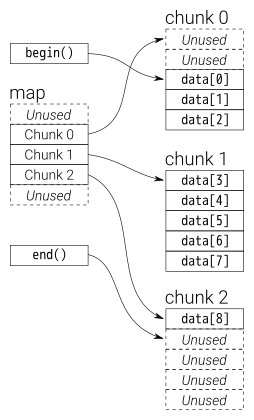
\includegraphics[height=8cm,keepaspectratio]{images/std-deque.png}

\end{frame}

% ----------------------------------------------------------------- %

\begin{frame}[fragile]
\frametitle{Do you remember \texttt{std::deque}?}
Although it's quite complex, it works not extremely slow in practice. It \textit{may be} good price for having non-invalidating iterators.\footnote{\href{https://baptiste-wicht.com/posts/2012/12/cpp-benchmark-vector-list-deque.html}{C++ benchmark - \texttt{std::vector} VS \texttt{std::list} VS \texttt{std::deque}}}

But don't forget: you won't be able to rely on contiguous element storing like in Rust!
\end{frame}

% ----------------------------------------------------------------- %

\begin{frame}[fragile]
\frametitle{\texttt{BTreeMap}\footnote{\href{https://doc.rust-lang.org/std/collections/struct.BTreeMap.html}{\texttt{BTreeMap} documentation}} and \texttt{BTreeSet}\footnote{\href{https://doc.rust-lang.org/std/collections/struct.BTreeSet.html}{\texttt{BTreeSet} documentation}}}
Rust also includes collections sorted by key: map and set.

\begin{itemize}
    \item<2-> There's a B-tree data structure inside. Thus it is cache-local and works fast on modern CPUs. Asymptotics for most operations are $O(\log_BN)$.
    \item<3-> Lecturer's humble opinion: these names are much better than \texttt{std::map} or \texttt{std::set} since they shows what data structure it uses. B-tree, hash table, cartesian tree are also maps and sets!
    \item<4-> \textbf{It is a logic error for a key to be modified in such a way that the key’s ordering relative to any other key changes while it is in the map}. The behavior resulting from such a logic error \textbf{is not specified} but \textbf{will not be undefined behavior}.
\end{itemize}
\end{frame}

% ----------------------------------------------------------------- %

\begin{frame}[fragile]
\frametitle{Do you remember \texttt{std::map} and \texttt{std::set}?}
In C++, we also have ordered map and set. Usually they are implemented using red-black trees.

\begin{itemize}
    \item<2-> If B-tree data structure is really cool, why don't we use it in C++ standard library, downgrading to red-black trees?
    \item<3-> \textit{Once again: iterator invalidation.}
    \item<4-> Since B-tree stores elements in chunks and have smaller depth, it way faster than regular BST.
    \item<5-> This really hurts! C++ don't have standard fast ordered map and set!
\end{itemize}
\end{frame}

% ----------------------------------------------------------------- %

\begin{frame}[fragile]
\frametitle{\texttt{HashMap}\footnote{\href{https://doc.rust-lang.org/std/collections/struct.HashMap.html}{\texttt{HashMap} documentation}} and \texttt{HashSet}\footnote{\href{https://doc.rust-lang.org/std/collections/struct.HashSet.html}{\texttt{HashSet} documentation}}}
What a language without hast table? Rust have two: \texttt{HashMap} and \texttt{HashSet}. Asymptotics are predictable.

\begin{itemize}
    \item<2-> This hash table is quite literally the fastest universal hash table in the world currently existing. It uses quadratic probing and SIMD lookup inside.
    \item<3-> More specifically, it's Rust port called Hashbrown of Google SwissTable written in C++. If you're interested in the algorithm, you can watch CppCon talk.\footnote{\href{https://www.youtube.com/watch?v=ncHmEUmJZf4}{CppCon 2017: Matt Kulukundis ``Designing a Fast, Efficient, Cache-friendly Hash Table, Step by Step''}}
    \item<4-> \textbf{It is a logic error for a key to be modified in such a way that the key's hash or its equality changes while it is in the map}. The behavior resulting from such a logic error \textbf{is not specified}, but \textbf{will not result in undefined behavior}.
\end{itemize}
\end{frame}

% ----------------------------------------------------------------- %

\begin{frame}[fragile]
\frametitle{Do you remember \texttt{std::unordered\_map} and \texttt{std::unordered\_set}?}
In C++, we also have unordered map and set. Usually they are implemented in some strange way.

\begin{itemize}
    \item<2-> Again: if Google Swiss table is really cool, why don't we use it in C++ standard library, donwgrading to some strange implementation?
    \item<3-> \textit{And once more: iterator invalidation!} At least it prevents us to use open addressing.
    \item<4-> This leads to not suitable for production standard library hash tables.
\end{itemize}
\end{frame}

% ----------------------------------------------------------------- %

\begin{frame}[fragile]
\frametitle{\texttt{BinaryHeap}\footnote{\href{https://doc.rust-lang.org/stable/std/collections/struct.BinaryHeap.html}{\texttt{BinaryHeap} documentation}}}
A priority queue implemented with a binary heap. \textbf{This will be a max-heap}. The same as in C++. Asymptotics are predictable.

\begin{itemize}
    \item<2-> Lecturer's humble opinion: this name is much better than \texttt{std::priority\_queue} since it shows what data structure it uses. For instance, binomial or fibonacci heaps are also priority queues!
    \item<3-> \textbf{It is a logic error for an item to be modified in such a way that the item’s ordering relative to any other item changes while it is in a heap}. The behavior resulting from such a logic error \textbf{is not specified} but \textbf{will not be undefined behavior}.
\end{itemize}
\end{frame}

% ----------------------------------------------------------------- %

\begin{frame}[fragile]
\frametitle{\texttt{LinkedList}\footnote{\href{https://doc.rust-lang.org/std/collections/struct.LinkedList.html}{\texttt{LinkedList} documentation}}}
A doubly-linked list with owned nodes. The same as in C++. Asymptotics are predictable.

\begin{itemize}
    \item You don't need it in almost any situation. It's slow and not memory efficient. Trust me.
    \item Since it's not C++, we don't have iterators pointing to elements. It's not convenient.
    \item Writing your list without unsafe is possible, but quite a challenge! Do it if you want to have a borrow checker as your best friend.\footnote{\href{https://rust-unofficial.github.io/too-many-lists/}{Learn Rust With Entirely Too Many Linked Lists}}
\end{itemize}
\end{frame}

% ----------------------------------------------------------------- %

\begin{frame}[c]
\centering\Huge\textbf{\texttt{String} and \texttt{\&str}}
\end{frame}

% ----------------------------------------------------------------- %

\begin{frame}[fragile]
\frametitle{\texttt{String}\footnote{\href{https://doc.rust-lang.org/std/string/struct.String.html}{\texttt{String} documentation}}}
A Rust way to store a string. \textbf{Totaly differs} from C++ \texttt{std::string}.

\begin{itemize}
    \item<2-> It's \textbf{UTF-8–encoded}.
    \item<3-> Growable like a \texttt{Vec}. It also made up of three components: a pointer to some bytes, a length, and a capacity. This even gives us many functions same to \texttt{Vec}.
    \item<4-> UTF-8 is a variable-width character encoding, so you cannot index it since it's UTF-8. To find N-th symbol, you should iterate over string, parsing code points.
\end{itemize}
\end{frame}

% ----------------------------------------------------------------- %

\begin{frame}[fragile,c]
\frametitle{\texttt{String} API}
\begin{minted}[fontsize=\small]{rust}
    struct String {
        vec: Vec<u8>,
    }

    impl String {
        fn new() -> String;
        fn with_capacity(capacity: usize) -> String;
        fn from_utf8(vec: Vec<u8>) -> Result<String, FromUtf8Error>;
        fn from_utf16(v: &[u16]) -> Result<String, FromUtf16Error>;
        fn into_bytes(self) -> Vec<u8>;
        fn as_bytes(&self) -> &[u8];
    }
\end{minted}
\end{frame}

% ----------------------------------------------------------------- %

\begin{frame}[fragile]
\frametitle{\texttt{String} in depth}
What will this code print?

\begin{minted}{rust}
    let s = String::from("привет");
    println!("{}", s.len());
\end{minted}
\end{frame}

% ----------------------------------------------------------------- %

\begin{frame}[fragile]
\frametitle{\texttt{String} in depth}
What will this code print?

\begin{minted}{rust}
    let s = String::from("привет");
    println!("{}", s.len());
\end{minted}

This outputs 12, since \texttt{.len()} gives count of \textit{bytes} in string.
\end{frame}

% ----------------------------------------------------------------- %

\begin{frame}[fragile]
\frametitle{\texttt{String} in depth}
To work directly with a string like in C++, you must convert it to \texttt{Vec<char>}

\begin{minted}{rust}
    let s = String::from("привет");
    let t = s.chars().collect::<Vec<_>>();
    println!("{:?}", t); // ['п', 'р', 'и', 'в', 'е', 'т']
\end{minted}

\texttt{.chars()} is function that creates iterator over chars of the string.
\end{frame}

% ----------------------------------------------------------------- %

\begin{frame}[fragile]
\frametitle{The \texttt{char} type}
The \texttt{char} type represents a single character.

More specifically, since ``character'' isn’t a well-defined concept in Unicode, \texttt{char} is a ``\textbf{Unicode scalar value}'', which is similar to, but not the same as, a ``\textbf{Unicode code point}''.
\end{frame}

% ----------------------------------------------------------------- %

\begin{frame}[fragile]
\frametitle{\texttt{char} type}
\begin{minted}{rust}
    let mut chars = "é".chars();
    // U+00e9: 'latin small letter e with acute'
    assert_eq!(Some('\u{00e9}'), chars.next());
    assert_eq!(None, chars.next());

    let mut chars = "é".chars();
    // U+0065: 'latin small letter e'
    assert_eq!(Some('\u{0065}'), chars.next());
    // U+0301: 'combining acute accent'
    assert_eq!(Some('\u{0301}'), chars.next());
    assert_eq!(None, chars.next());
\end{minted}
\end{frame}

% ----------------------------------------------------------------- %

\begin{frame}[fragile]
\frametitle{\texttt{char} type}
The size of \texttt{char} is always 4 bytes:

\begin{minted}{rust}
    assert_eq!(std::mem::size_of::<char>(), 4);
\end{minted}
\end{frame}

% ----------------------------------------------------------------- %

\begin{frame}[fragile]
\frametitle{\texttt{\&str}}
\texttt{\&str} is a slice type of \texttt{String}, similar to \texttt{std::string\_view}. Just like:

\begin{minted}{rust}
    let vec = vec![1, 2, 3, 4];
    let vec_slice = &vec[1..3]; // &[2, 3]
    let s = String::from("hello");
    let s_slice = &s[1..3]; // "el"
\end{minted}
\end{frame}

% ----------------------------------------------------------------- %

\begin{frame}[fragile]
\frametitle{\texttt{\&str}}
Ok, let's take a UTF-8 slice!

\begin{minted}{rust}
    let s = String::from("привет");
    let s_slice = &s[1..3];
\end{minted}
\end{frame}

% ----------------------------------------------------------------- %

\begin{frame}[fragile]
\frametitle{\texttt{\&str}}
Ok, let's take a UTF-8 slice!

\begin{minted}{rust}
    let s = String::from("привет");
    let s_slice = &s[1..3];
    // thread 'main' panicked at 'byte index 1 is
    // not a char boundary; it is inside 'п'
    // (bytes 0..2) of `привет`'
\end{minted}
\end{frame}

% ----------------------------------------------------------------- %

\begin{frame}[fragile]
\frametitle{\texttt{\&str}}
Ok, let's take a UTF-8 slice!

\begin{minted}{rust}
    let s = String::from("привет");
    let s_slice = &s[1..3];
    // thread 'main' panicked at 'byte index 1 is
    // not a char boundary; it is inside 'п'
    // (bytes 0..2) of `привет`'
\end{minted}

That means \texttt{\&str} also have a UTF-8 invariant checked at runtime.
\end{frame}

% ----------------------------------------------------------------- %

\begin{frame}[fragile]
\frametitle{\texttt{\&str}}
As a string slice, \texttt{\&str} have most functions \texttt{String} have:

\begin{minted}{rust}
    fn as_bytes(&self) -> &[u8];
    fn chars(&self) -> Chars<'_>;
    fn trim(&self) -> &str;
    fn split<'a, P>(&'a self, pat: P) -> Split<'a, P>;
    fn replace<'a, P>(&'a self, from: P, to: &str) -> String;
    // And so on
\end{minted}
\end{frame}

% ----------------------------------------------------------------- %

\begin{frame}[fragile]
\frametitle{\texttt{\&str}}
All string constants are \texttt{\&str}.

\begin{minted}{rust}
    let s: &str = "Hello world!";
    let t1 = s.to_string();
    let t2 = s.to_owned(); // The same as t1
\end{minted}
\end{frame}

% ----------------------------------------------------------------- %

\begin{frame}[c]
\centering\Huge\textbf{\texttt{Box} and \texttt{Rc}}
\end{frame}

% ----------------------------------------------------------------- %

\begin{frame}[fragile]
\frametitle{\texttt{Box}}
We are already familiar with \texttt{Box} type. Let's check one advanced function:

\begin{minted}{rust}
    fn leak<'a>(b: Box<T, A>) -> &'a mut T;
    fn into_raw(b: Box<T, A>) -> *mut T;
\end{minted}

Example:

\begin{minted}{rust}
    let x = Box::new(41);
    let static_ref: &'static mut usize = Box::leak(x);
    *static_ref += 1;
    assert_eq!(*static_ref, 42);
\end{minted}
\end{frame}

% ----------------------------------------------------------------- %

\begin{frame}[fragile]
\frametitle{\texttt{Box}}
\textbf{But stop!} Rust is the safe language, no memory unsafety, no undefined behavior, what's wrong!?

\visible<2->{
    \textit{In reality, when you're creating global objects or interacting with other languages, you \textbf{have to} leak objects. Moreover, it's \textbf{safe} to leak memory, just not good!}
}
\end{frame}

% ----------------------------------------------------------------- %

\begin{frame}[fragile]
\frametitle{\texttt{Rc}}
\texttt{Rc} is single-threaded reference-counting pointer. ``\texttt{Rc}'' stands for ``Reference Counted''.

\begin{minted}{rust}
    let rc = Rc::new(());
    let rc2 = rc.clone(); // Clones Rc, not what inside!
    let rc3 = Rc::clone(&rc); // The same
\end{minted}

\texttt{Rc} is dropped when all instances of \texttt{Rc} are dropped.

Primary functions:

\begin{minted}{rust}
    fn get_mut(this: &mut Rc<T>) -> Option<&mut T>;
    fn downgrade(this: &Rc<T>) -> Weak<T>;
    fn weak_count(this: &Rc<T>) -> usize;
    fn strong_count(this: &Rc<T>) -> usize;
\end{minted}
\end{frame}

% ----------------------------------------------------------------- %

\begin{frame}[fragile]
\frametitle{\texttt{Rc}}
References to the variable inside \texttt{Rc} are controlled at runtime:

\begin{minted}{rust}
    let mut rc = Rc::new(42);
    println!("{}", *rc);

    *Rc::get_mut(&mut rc).unwrap() -= 41;
    println!("{}", *rc);

    let mut rc1 = rc.clone();
    println!("{}", *rc1);
    // thread 'main' panicked at 'called `Option::unwrap()`
    // on a `None` value'
    // *Rc::get_mut(&mut rc1).unwrap() -= 1;
\end{minted}

\texttt{get\_mut} guarantees that it will return mutable reference only if there's only one pointer. If there are more, you won't have a chance to modify \texttt{Rc}.
\end{frame}

% ----------------------------------------------------------------- %

\begin{frame}[fragile]
\frametitle{\texttt{Weak}}
\texttt{Rc} is a \textbf{strong} pointer, while \texttt{Weak} is a \textbf{weak} pointer. Both of them have \textit{ownership over allocation}, but only \texttt{Rc} have \textit{ownership over the value inside}:

You can upgrade \texttt{Weak} to \texttt{Rc}:

\begin{minted}{rust}
    fn upgrade(&self) -> Option<Rc<T>>;
\end{minted}
\end{frame}

% ----------------------------------------------------------------- %

\begin{frame}[fragile,c]
\frametitle{\texttt{Weak}}
\begin{minted}{rust}
    let rc1 = Rc::new(String::from("string"));
    let rc2 = rc1.clone();
    let weak1 = Rc::downgrade(&rc1);
    let weak2 = Rc::downgrade(&rc1);
    drop(rc1); // The string is not deallocated
    assert!(weak1.upgrade().is_some());
    drop(weak1); // Nothing happens
    drop(rc2); // The string is deallocated
    assert_eq!(weak2.strong_count(), 0);
    // If no strong pointers remain, this will return zero.
    assert_eq!(weak2.weak_count(), 0);
    assert!(weak2.upgrade().is_none());
    drop(weak2); // The Rc is deallocated
\end{minted}
\end{frame}

% ----------------------------------------------------------------- %

\begin{frame}[fragile]
\frametitle{\texttt{Arc}}
There's also \texttt{Arc} - a thread-safe reference-counting pointer. \texttt{Arc} stands for ``Atomically Reference Counted''.

We'll need it to share data safely across threads in the future.
\end{frame}

% ----------------------------------------------------------------- %

\begin{frame}[fragile]
\frametitle{Conclusion}
\begin{itemize}
    \item We studied API of Option and Result.
    \item Get acquainted with default collections.
    \item Learned about smart pointers in Rust.
\end{itemize}
\end{frame}

% ----------------------------------------------------------------- %

\end{document}
